\documentclass[a4paper,
fontsize=11pt,
%headings=small,
oneside,
numbers=noperiodatend,
parskip=half-,
bibliography=totoc,
final
]{scrartcl}

\usepackage{synttree}
\usepackage{graphicx}
\setkeys{Gin}{width=.4\textwidth} %default pics size

\graphicspath{{./plots/}}
\usepackage[ngerman]{babel}
\usepackage[T1]{fontenc}
%\usepackage{amsmath}
\usepackage[utf8x]{inputenc}
\usepackage [hyphens]{url}
\usepackage{booktabs} 
\usepackage[left=2.4cm,right=2.4cm,top=2.3cm,bottom=2cm,includeheadfoot]{geometry}
\usepackage{eurosym}
\usepackage{multirow}
\usepackage[ngerman]{varioref}
\setcapindent{1em}
\renewcommand{\labelitemi}{--}
\usepackage{paralist}
\usepackage{pdfpages}
\usepackage{lscape}
\usepackage{float}
\usepackage{acronym}
\usepackage{eurosym}
\usepackage[babel]{csquotes}
\usepackage{longtable,lscape}
\usepackage{mathpazo}
\usepackage[normalem]{ulem} %emphasize weiterhin kursiv
\usepackage[flushmargin,ragged]{footmisc} % left align footnote
\usepackage{ccicons} 

%%%% fancy LIBREAS URL color 
\usepackage{xcolor}
\definecolor{libreas}{RGB}{112,0,0}

\usepackage{listings}

\urlstyle{same}  % don't use monospace font for urls

\usepackage[fleqn]{amsmath}

%adjust fontsize for part

\usepackage{sectsty}
\partfont{\large}

%Das BibTeX-Zeichen mit \BibTeX setzen:
\def\symbol#1{\char #1\relax}
\def\bsl{{\tt\symbol{'134}}}
\def\BibTeX{{\rm B\kern-.05em{\sc i\kern-.025em b}\kern-.08em
    T\kern-.1667em\lower.7ex\hbox{E}\kern-.125emX}}

\usepackage{fancyhdr}
\fancyhf{}
\pagestyle{fancyplain}
\fancyhead[R]{\thepage}

% make sure bookmarks are created eventough sections are not numbered!
% uncommend if sections are numbered (bookmarks created by default)
\makeatletter
\renewcommand\@seccntformat[1]{}
\makeatother


\usepackage{hyperxmp}
\usepackage[colorlinks, linkcolor=black,citecolor=black, urlcolor=libreas,
breaklinks= true,bookmarks=true,bookmarksopen=true]{hyperref}
%URLs hart brechen
\makeatletter 
\g@addto@macro\UrlBreaks{ 
  \do\a\do\b\do\c\do\d\do\e\do\f\do\g\do\h\do\i\do\j 
  \do\k\do\l\do\m\do\n\do\o\do\p\do\q\do\r\do\s\do\t 
  \do\u\do\v\do\w\do\x\do\y\do\z\do\&\do\1\do\2\do\3 
  \do\4\do\5\do\6\do\7\do\8\do\9\do\0} 
% \def\do@url@hyp{\do\-} 
\makeatother 

%meta
%meta

\fancyhead[L]{K. Schuldt \\ %author
LIBREAS. Library Ideas, 33 (2018). % journal, issue, volume.
\href{http://nbn-resolving.de/}
{}} % urn 
% recommended use
%\href{http://nbn-resolving.de/}{\color{black}{urn:nbn:de...}}
\fancyhead[R]{\thepage} %page number
\fancyfoot[L] {\ccLogo \ccAttribution\ \href{https://creativecommons.org/licenses/by/3.0/}{\color{black}Creative Commons BY 3.0}}  %licence
\fancyfoot[R] {ISSN: 1860-7950}

\title{\LARGE{Einige Anmerkungen zur Stimmung des Personals am Arbeitsplatz Bibliothek}} % title
\author{Karsten Schuldt} % author

\setcounter{page}{1}

\hypersetup{%
      pdftitle={Einige Anmerkungen zur Stimmung des Personals am Arbeitsplatz Bibliothek},
      pdfauthor={Karsten Schuldt},
      pdfcopyright={CC BY 3.0 Unported},
      pdfsubject={LIBREAS. Library Ideas, 33 (2018).},
      pdfkeywords={Bibliotheksarbeit, Mitarbeiterführung, Lohnarbeit},
      pdflicenseurl={https://creativecommons.org/licenses/by/3.0/},
      pdfcontacturl={http://libreas.eu},
      baseurl={http://libreas.eu},
      pdflang={de},
      pdfmetalang={de}
     }



\date{}
\begin{document}

\maketitle
\thispagestyle{fancyplain} 

%abstracts

%body
\hypertarget{drei-szenen}{%
\section*{Drei Szenen}\label{drei-szenen}}

Das Thema dieses Essays ist, wie noch gezeigt wird, schwierig zu
konkretisieren. Insoweit scheint es passend, erzählerisch mit drei
Szenen, an denen ich beteiligt war, zu beginnen. Szenen wie diese haben
mich zum Thema gebracht.

\hypertarget{erste-szene-ist-doch-alles-gut.}{%
\subsection*{Erste Szene: Ist doch alles
gut.}\label{erste-szene-ist-doch-alles-gut.}}

Ende 2017, im Büro eines Kollegen. Er erläutert mir die Gründe für die
Ablehnung eines internen Antrags. An der HTW Chur, an der ich als
Wissenschaftlicher Mitarbeiter tätig bin, kann man genauso wenig wie an
anderen Fachhochschulen einfach nach Interesse oder gesellschaftlichem
Bedarf forschen. Vielmehr muss alles irgendwie finanziert werden. Unter
anderem gibt es dafür, ebenfalls wie an anderen Fachhochschulen, interne
Anträge, aufgrund derer hochschuleigene Kommissionen intern
Forschungsmittel vergeben. Diese Kommissionen bestehen oft aus
Professorinnen und Professoren aller Institute der Hochschule, was auch
heisst, dass man jedesmal Dinge, die im eigenen Feld klar sind, neu
erklären muss, weil die Kolleginnen und Kollegen in den anderen
Instituten sich halt vor allem mit ihren eigenen Feldern auskennen.

Ich hatte in der letzten Runde einen Antrag eingereicht, in dem ich
vorschlug, die Prozesse zur Personalgewinnung von
Gedächtniseinrichtungen (Bibliotheken, Museen, Archive) zu untersuchen.
Es scheint eine absurde Zeit zu sein: In vielen dieser Einrichtungen im
deutschsprachigen Raum scheint mehr und mehr die Angst umzugehen, kein
geeignetes Personal zu finden. Stellen werden mehrfach ausgeschrieben,
einmal gewonnenes Personal soll unbedingt gehalten werden, auf
Konferenzen und anderen Treffen wird sich Sorgen gemacht, ob sich
überhaupt noch jemand auf die jetzigen und zukünftigen Ausschreibungen
bewerben wird. Auf der anderen Seite gibt es viele unzufriedene
Menschen, die ein Interesse an solchen Stellen haben, die Ausbildungen
für diese Jobs absolviert haben, aber die seit Jahren nicht eingestellt
werden. Das ist selbstverständlich schwierig zu zeigen, aber wer sich im
Feld auskennt wird Dutzende solcher Personen kennen.

Redet man mit diesen über ihre Erfahrungen bei Bewerbungen für Stellen
in Gedächtniseinrichtungen, wird auch eine Enttäuschung mit den
Bewerbungsprozessen selber deutlich: Langsam, undurchsichtig, unklar,
wieso Ablehnungen ausgesprochen werden; wenn eingeladen, dann als
Bittstellerinnen und Bittsteller behandelt oder in Bewerbungsgesprächen
mit Fragen konfrontiert, bei denen man sich persönlich nicht ernst
genommen fühlt (oft, weil sie im ersten Semester Studium oder ersten
Jahr Ausbildung behandelt werden). Alles in allem: Viel Frust.\footnote{Ein
  Grund für meine Beschäftigung mit dem Thema ist auch mein eigener,
  steigender Frust mit diesen, für mich seit Jahren nicht erfolgreichen
  Bewerbungsverfahren. Erst dachte ich, es läge an mir. Aber nach
  einigen Jahren erfolgloser Bewerbungen stiess ich darauf, dass ich zum
  Beispiel aus meinem Studium der Bibliothekswissenschaft wohl mehr
  Menschen kenne, die ähnliche Geschichten und Frustrationen kennen, als
  solche, die heute erfolgreich und glücklich in Bibliotheken arbeiten.}

Gleichzeitig gibt es immer wieder Geschichten von Menschen, die in
Gedächtnisinstitutionen offenbar auf die falschen Positionen gelangt
sind, oft ohne wirkliche eigene Schuld. In Museen in der Schweiz gab es,
so wird unter der Hand berichtet, mehrfach Fälle, wo fachlich vollkommen
qualifizierte Personen auf Leitungspositionen eingesetzt wurden und dann
im Bereich Management, gerade von Personal oder Finanzen, scheiterten.
Über diese Fälle wird diskutiert, aber kaum publiziert. Im Kleineren
hört man ähnliches aber auch aus Bibliotheken und Archiven. Ist man
persönlich betroffen, ist dies individuell alles sehr frustrierend. Aber
aus der Sicht der angewandten Forschung scheint es auch ein
interessantes Problem darzustellen, das zu untersuchen und vielleicht
sogar zu lösen, motivierend wäre. (Und das in der Logik der
Fachhochschulen, in denen alles finanziert werden muss, sogar
Beratungsaufträge einbringen könnte.)

Sicher: Das ist alles sehr unfundiert, ist Hören-Sagen, eigenes Erleben,
keine fundierte Problembeschreibung. Aber man sollte die notwendige
Qualität von internen Anträgen an Fachhochschulen nicht überschätzen. Es
geht darum, zu zeigen, dass da ein Thema (und eine
Drittmittelfinanzierung) existieren könnte.

Doch dieser spezifische interne Antrag wurde abgelehnt. Diese Ablehnung
erläuterte mir der Kollege, welcher die Sitzungen der Kommission
besucht, noch einmal genauer. Das Hauptargument war, dass einfach nicht
geglaubt wurde, dass die Situation in Gedächtniseinrichtungen schlecht
wäre. Davon hätte man in der HTW Chur noch nie gehört, bei allen
Kontakten zu Bibliotheken, Archiven und Museen. Ausserdem gibt es eine
regelmässige Umfrage unter Absolventinnen und Absolventen und die seien
mit ihren Jobs nach dem Studium sehr zufrieden. Schon während dieser
Szene hatte ich das Gefühl, dass wir uns offenbar in unterschiedlichen
Welten bewegen. Ich kenne vor allem Einrichtungen, die sich Sorgen
machen (die sogar zum Teil der Hochschule Aufträge geben, weil sie keine
eigenes Personal dafür finden) und Menschen, die frustriert sind, weil
sie nicht ins System hineinkommen oder aber im System sind, aber nicht
da, wo sie sein wollen oder aber auch schon wieder aufgeben und in
andere Berufsfelder gewechselt haben. Aber offenbar ist das nicht das
Bild, dass andere vom Feld der Gedächtnisinstitutionen haben. Wie kann
das sein?

Im Anschluss an dieses Gespräch habe ich noch einmal andere Personen,
die mehr mit Gedächtniseinrichtungen zu tun haben, gefragt. Diese
bestätigten mir, dass meine Sicht vielleicht etwas übertrieben negativ
ist, aber sie es eher so wahrnehmen, wie ich. Offenbar gibt es zwei
Welten.

\hypertarget{zweite-szene-man-darf-sich-nicht-entwickeln.}{%
\subsection*{Zweite Szene: Man darf sich nicht
entwickeln.}\label{zweite-szene-man-darf-sich-nicht-entwickeln.}}

Mitte 2017, Gespräch mit einem der Absolventen einer der Hochschulen mit
bibliothekarischen Studiengängen im deutschsprachigen Raum. Er ist
frustriert. Angestellt in einer Filiale einer Stadtbibliothek in einer
grösseren Stadt hatte er das Studium offenbar auch gewählt, um
interessante Aufgaben übernehmen zu können. Als eine Position im
gleichen Bibliothekssystem ausgeschrieben wurde, die solche Aufgaben
versprach, wurde ihm von seiner Filialleitung mehr oder minder
untersagt, sich zu bewerben, obwohl das genau sein Interesse war. Die
Begründung: Die Filialleitung wollte ihn mit seinen Fähigkeiten
behalten. Dabei ist diese Stadtbibliothek eigentlich dafür bekannt ist,
offen und innovativ zu sein. Aber offenbar nicht für ihn. Er liess sich
das gefallen, weil er sein Studium erst einmal abschliessen wollte. Dann
passierte das ganze noch einmal.

Seine Lösung war, sich nach dem Ende des Studiums in ein gänzlich
anderes Bibliothekssystem auf eine gänzlich andere Stelle zu bewerben.
Mit Erfolg, aber eingeschränkter Begeisterung, da er persönliche
Verbindungen zu der Stadt hat, in der er vorher arbeitete und jetzt
regelmässig rund hundert Kilometer pendeln würde.

Sporadische Kontakte zu ehemaligen Studierenden erbringen immer wieder
auch solche Geschichten von Frustration. Immer mit Einschränkungen, es
gibt bestimmt viele Leben und Schicksale, die frustrierender sind.. Aber
Unzufriedenheit mit der eigenen Arbeit, der Position in der man sich
befindet, den wenigen Aufgaben, die man lösen darf, scheint im
Arbeitsalltag der Bibliotheken eher normal zu sein. Oft sind auch
Erwartungen enttäuscht, wenn Menschen zwar studiert haben, aber nach dem
Studium weiter nur die Stelle besetzen dürfen, die sie vorher schon
besetzten - nur jetzt mit akademischen Abschluss. Aufällig scheint mir,
wie viele ehemalige Studierende entweder das Bibliothekswesen nach dem
Studium hinter sich lassen oder aber relativ schnell die Stellen
wechseln.

Insoweit scheint die Geschichte des Absolventen eine unter vielen.

\hypertarget{dritte-szene-das-wird-nur-schlimmer.}{%
\subsubsection*{Dritte Szene: Das wird nur
schlimmer.}\label{dritte-szene-das-wird-nur-schlimmer.}}

Anfang 2018, eine Bezirkszentralbibliothek einer deutschen Grossstadt.
Mit einer anderen LIB\-REAS-Redakteurin bin ich dort, eigentlich um etwas
zu arbeiten; aber wir gehen vorher noch durch die Bibliothek. Dies war
die Stammbibliothek der Redakteurin, bevor sie vor einigen Monaten
fortzog. In einem Raum räumt eine Bibliothekarin Medien ein. Die
ehemalige Stammnutzerin ist verwundert, dass die DVDs jetzt hier stehen.
Sie fragt die Bibliothekarin, seit wann das so ist. Denn eigentlich
standen hier die Kunstbücher.

Wir weisen uns zu Beginn nicht explizit als vom Fach aus. Vielleicht ist
es aber offensichtlich. Zumindest nimmt die Bibliothekarin der
Stadtteilbibliothek die eine Frage zum Anlass, um über die Situation zu
klagen. Sie müsse jetzt aufräumen, obwohl sie andere Aufgaben hätte,
sowohl von der Ausbildung her als auch von ihrer Position in der
Bibliothek. Eigentlich sollten dies FaMIs machen, nicht
Bibliothekarinnen mit Diplom kurz vor der Rente - sie selber ist kurz
vor der Rente, meint deshalb, dass es sie jetzt nicht mehr so sehr
trifft. Aber für die jüngeren Kolleginnen und Kollegen sieht sie alles
schlimmer werden. Zu viele neue Aufgaben, zu wenig Personal, zu wenig
Unterstützung. Dann geht sie auch noch auf Spezifika der politischen
Situation in der Stadt ein (einer sowohl von der Regierung und den
Wahlergebnissen als auch vom Ruf und Lebensgefühl her \enquote{linken
Stadt}, notabene), die für die Bibliotheken aber auch für andere
Kultureinrichtungen desaströs wäre. Dabei, das muss man sagen, ist die
Bibliothek in einem neu renovierten, grosszügigen Gebäude untergebracht.
Die Nutzerinnen und Nutzer sind ruhig und arbeiten vor sich hin. Die
Bestände sehen nicht verbraucht und ungeordnet aus. Auf den ersten Blick
scheint alles einigermassen in Ordnung.

Überraschend ist, wie offen sich die Bibliothekarin zwei wildfremden
Personen gegenüber zu ihrer Arbeitssituation - und nicht nur ihrer
persönlichen, sondern der in der Bibliothek insgesamt - äussert. Hier
scheint sich sehr viel aufgestaut zu haben. Dabei ist auch zu merken,
dass es nicht gegen ihre direkten Kolleginnen und Kollegen geht. Die
scheinen nicht der Grund für ihre Frustrationen zu sein.

Gleichzeitig ist das keine überraschende Szene. Ich habe ähnliche
Gespräche in den letzten Jahren in unterschiedlichen deutschen,
schweizerischen und österreichischen Bibliotheken in grossen Städten und
in kleinen Gemeinden geführt. Nicht regelmässig bei jedem Besuch, aber
doch so oft, dass sie mir nicht mehr wie einzelne, individuelle Fälle
vorkommen, sondern als Anzeichen für ein strukturelles Problem.

\hypertarget{die-unuxfcbersichtliche-gesamtsituation}{%
\section*{Die unübersichtliche
Gesamtsituation}\label{die-unuxfcbersichtliche-gesamtsituation}}

Die Frage, der ich mich nähere: Wie ist die Stimmung im
bibliothekarischen Personal eigentlich? Mich interessiert das
persönlich\footnote{Weil ich dieses Personal mit ausbilde und deshalb
  meine, eine gewisse Verantwortung dafür zu haben, dass sie auch etwas
  aus dieser Ausbildung machen können. Und weil ich eigentlich selber,
  wie oben geschildert, seit Jahren gerne Teil dieses Personals werden
  möchte.} und aus forschender Perspektive.

Die Diskussionen im Bibliothekswesen sind bekanntlich von Sichten auf
sich selbst geprägt. Die Frage, wie Bibliotheken in der Öffentlichkeit
oder Teilen der Öffentlichkeit (zum Beispiel bei Jugendlichen) gesehen
werden; die Frage, welche Stereotype über Bibliotheken existieren; die
Frage, wie modern Bibliotheken sind oder wie sie modern werden können -
all das interessiert offenbar, wenn man die bibliothekarische Literatur
anschaut. Aber die Situation des Personals selber, also was die
Bibliothekarinnen und Bibliothekare eigentlich wollen, machen, im Alltag
fühlen, woran sie verzweifelt und was sie stolz macht, das ist fast nie
ein Thema. Obwohl es für das Funktionieren einer Bibliothek (sowohl
verstanden als \enquote{funktioniert so, wie es soll} als auch
soziologisch als \enquote{wie kommt es, dass die Institution
funktioniert, wie sie funktioniert?}) wichtig ist, was das Personal
macht und wieso.

Mein Eindruck ist, wie schon erläutert, dass Menschen auf vielen Seiten
frustriert sind. Und das in einer komischen Situation: Nicht so sehr mit
dem Job an sich, auch weniger mit den Kolleginnen und Kollegen, sondern,
well, mit der Gesamtsituation. Oder anders: Den Strukturen, die zu
massenhaften Frustrationen führen (persönlichen, aber auch
organisationellen, wenn die Angst besteht, kein geeignetes Personal mehr
zu finden). Leider hilft die bisherige Forschung aber nicht weiter,
dieses Gefühl zu belegen oder zu widerlegen. Das Thema selber wird kaum
behandelt, schon gar nicht für den deutschsprachigen Raum.

Der umfangreichste und systematischste Text zum Thema scheint der von
Davis Kendrick (2017) zu sein, die -- allerdings für die USA -- für
akademischen Bibliotheken etwas untersuchte, was sie \enquote{Low Morale
Experience} nennt. Diese würde sich dadurch auszeichnen, dass
Angestellte systematisch (also nicht manchmal, sondern ständig, quasi
als Grundgefühl) unzufrieden mit ihrem Arbeitsplatz seien, sich
unterfordert oder aber ausgebeutet, nicht in ihren Kompetenzen beachtet
oder gar ständig beleidigt fühlen würden. Dies würde zu einer schlechten
Arbeitsmoral bei den betroffenen Personen führen, aber kein rein
individuelles Problem sein, sondern sich auch auf die Arbeitskultur der
ganzen Organisation auswirken.

Im Literaturbericht ihres Artikels hält sie fest, dass es auch in der
englischsprachigen bibliothekarischen Literatur praktisch keine Texte,
Studien oder Diskussionen zum Thema gibt. (Davis Kendrick 2017:847-848)
Einzelne Themen, die mit einer Low Morale Experience verbunden werden --
\enquote{workplace bullying, incivility, toxicity, and burnout} (Davis
Kendrick 2017:847) --, wurden in den letzten Jahren behandelt. (Ryan
2016; Wheeler 2016; Alabi 2015; Hecker 2007) Aber auch dann sehr auf die
Frage abzielend, wie diese zu verhindern seien, nicht unter der
Fragestellung, warum sie überhaupt auftreten.

Davis Kendrick führte mit 20 Bibliothekarinnen und Bibliothekaren -- die
auf eine Einladung zur Teilnahme an der Studie reagiert hatten, welche
über mehrere bibliothekarische Mailinglisten verteilt wurde --
Interviews durch. Das ist keine grosse Zahl und auch keine
repräsentative Auswahl, aber es ist eine Basis für eine explorative
Studie. Zudem deckte die Auswahl eine grosse Bandbreite (new, mid-career
und experienced librarians; aus unterschiedlichen Regionen und
Bibliothekstypen und so weiter) ab. Die Interviews zeichnen ein ganz
erschreckendes Bild: Bibliothekarinnen berichten davon, sich emotional
missbraucht zu fühlen und als Angestellte vernachlässigt zu werden.
Viele berichten von langen Zeiträumen, in denen sie sich so fühlten.
Zwar gab es auch eine ganze Anzahl, die mit der Situation umzugehen
lernten und sie irgendwann verlassen oder verändern konnten, aber nicht
ohne eine lange Zeit unter ihr zu leiden. Und in dieser Menge scheint es
sich auch nicht um Einzelfälle zu handeln, sondern nur um einigen von
vielen Betroffenen, die sich äusserten. Gründe für diese Low Morale
Experiences waren -- in dieser Reihenfolge -- Inkompetenz des
Managements, persönliche Konflikte, verbale Übergriffe, Veränderungen im
Management, emotionaler Missbrauch und Arbeitsüberlastung.

Diese Situationen hatten für die Betroffenen und die Institutionen
relevante Konsequenzen: Sie selber mussten mit langfristig wirkenden
Gefühlen von Angst und Unmut umgehen, entwickelten eine Haltung von
ständiger Skepsis und ständigem Misstrauen ihren Vorgesetzten sowie
Kolleginnen und Kollegen gegenüber, hatten weniger Vertrauen darin,
überhaupt ihre tägliche Arbeit bewältigen zu können, mussten mit
physischen und psychischen Problemen umgehen. Viele entwickelten ihre
Karriere wegen dieser Situation auch nicht weiter.\footnote{Zu bedenken
  ist zudem, dass Davis Kendrick nur Personen erreichte, die
  bibliothekarische Mailinglisten lasen. Diejenigen, welche die
  Profession vielleicht aufgrund ihrer Erfahrungen verlassen haben,
  konnte sie gar nicht erst erreichen.} Für die Einrichtungen hiess das,
dass sie Personal hatten, welches mehr mit sich und der eigenen
Situation beschäftigt war, als der eigentlichen Arbeit; das weit weniger
engagiert und produktiv war, als es hätten sein können. Das kann auch
für die betroffenen Bibliotheken als Institutionen nicht gut sein.

Aber offenbar gilt auch für die Leitungsebenen in Bibliotheken nicht,
dass alles gut ist. Funge et al. (2017) untersuchten die Einstellungen
und Erfahrungen von Leitungspersonal, wieder in den USA, diesmal mit
einer Umfrage. Grundsätzlich war deren Gefühl besser als bei den von
Davis Kendrick Interviewten. Aber auch hier gab es Klagen über
Mikroaggressionen des Personals gegenüber den Personen mit
Leitungsfunktionen (etwas mehr, wenn das Bibliothekspersonal
\enquote{non-minority groups} angehörte (Funge et al.~2017:732-733)),
inklusive expliziter Verweigerungshaltungen des Personals, vor allem der
Verweigerung von Veränderung. Die Autorinnen und Autoren dieser Studie
empfehlen, dass Bibliotheken ein gemeinsames Zusammengehörigkeitsgefühl
-- also von Personal und Leitung -- fördern sollten, um negative Effekte
von Friktionen zwischen diesen Gruppen entgegenzuwirken. Auch hier ist
eine Vermutung, dass man es nicht empfehlen müsste, wenn es normal
wäre.\footnote{Vorschläge, wie etwas im Bereich Arbeitskultur (weniger
  Bullying, weniger Stress, weniger Barrieren für den Zugang in das
  Bibliothekswesen und Karrierewege in diesem und so weiter) zu
  bewerkstelligen wäre, finden sich in der US-amerikanischen
  Bibliotheksliteratur offenbar recht oft. So, als wäre es etwas, was
  noch breitflächig erreicht werden muss. Siehe zum Beispiel Eads
  (2017), Hecker (2007), Carlton (2017). Auch das vom Titel her mehr
  versprechende \enquote{The Dysfunctional Library} (Henry, Eshleman \&
  Moniz 2018; kurzgefasst auch: Henry et al.~2018) ist eigentlich vor
  allem eine Anleitung, wie es besser zu machen wäre. Dieses Buch
  überträgt -- beschränkt auf die US-amerikanische Gesellschaft -- vor
  allem Studien aus anderen Bereichen auf Bibliotheken, immer mit der
  Überzeugung, dass, wenn es in anderen schlecht mit der
  Arbeitsplatzkultur und der Zivilisiertheit im Umgang der Menschen
  untereinander steht, es auch in der Bibliothek schlecht stehen würde.}

In der Studie von Houston und Paganelli (2015) ging es -- wieder per
Umfrage -- um die emotionale Reaktion von US-amerikanischen
Schulbibliothekarinnen und -bibliothekaren auf Veränderungen. Auch diese
waren grundsätzlich eher schlecht. Eine kleine Gruppe freute sich über
Veränderungen, viele kamen mit der Zeit mit den Veränderungen zurecht,
wenn sie dann einmal eingeführt waren. Je mehr sich die Personen selber
dazu in der Lage sahen, Veränderungen anzustossen, um so eher fühlten
sie sich gut mit ihnen (\enquote{optimistic, excited, confident}). Aber
wenn sie das Gefühl hatten, und das hatten die meisten, dass die
Veränderungen ihnen von ausserhalb aufgenötigt wurden, dann hatten sie
eine negative emotionale Reaktion (\enquote{angry, cynical, anxious,
worried, discouraged}). Angesichts dessen, dass sich selbstverständlich
auch Bibliotheken ständig ändern, ist das keine gute Situation. Zu
vermuten ist auch erst einmal nicht, dass die Befragten in Bibliotheken
per se ängstlicher sind als andere, sondern dass die Struktur der
Schulbibliotheken, also ihr Arbeitsplatz, etwas damit zu tun haben.
Ansonsten wäre das Ergebnis nicht so durchgängig schlecht.

Neben diesen Problemen, welche innerhalb der Institutionen entstehen,
ist das Bibliothekswesen eine Profession, in der viele Kolleginnen und
Kollegen ständig Kontakt mit Nutzerinnen und Nutzern haben. (Peet 2017)
Das ist soziale Arbeit und in vielen Fällen offenbar auch eine
Situation, die zu Problemen führen kann. In zwei ähnlichen Texten
(Carlton 2017; Ford 2017) berichtete zum Beispiel das American Libraries
Magazine von einem Vortrag auf der ALA-Konferenz 2017, bei dem zwei
Kolleginnen eine Studie über sexuelle Belästigungen im Bibliotheksalltag
vorstellten und Vorschläge machten, wie in solchen Situationen gehandelt
werden kann. Ihre Studie umfasste immerhin 173 Personen, die über solche
Fälle berichteten. Insoweit kann vermutet werden, dass auch dies ein
strukturelles Problem darstellt, keine Einzelfälle. Dass das Buch von
Martin Eichhorn (Eichhorn 2015) zu \enquote{Konflikt- und
Gefahrensituationen in Bibliotheken}, welches sich eigentlich liest, wie
aus einer anderen, gefährlicheren Welt, jetzt schon in der dritten
Auflage vorliegt und Eichhorn auch weiter Seminare zum Thema
anbietet,\footnote{Vergleiche
  \url{http://www.martin-eichhorn.berlin/Fuer-Bibliothekspersonal}.}
wird seinen Grund auch darin haben, dass eine ganze Anzahl von
Kolleginnen und Kollegen solche Situationen -- die im Buch Situationen
im Umgang mit Nutzerinnen und Nutzern meinen -- als real wahrnimmt.

Daneben gibt es aber auch eine Anzahl von Texten, die gut zur Frage
dieses Textes selber passen würden, da sie sich mit der Zufriedenheit
des Personals in Bibliotheken mit der eigenen Arbeit befassen; die aber
einen Forschungsaufbau aufweisen, in dem die negativen Haltungen, die
zum Beispiel Davis Kendrick (2017) erwähnt, gar nicht auftauchen können.
Oyovwe Tinuoye, Omeluzor und Oji Akpojotor (2016) untersuchten zum
Beispiel in zwei nigerianischen Bundesstaaten mit einer Umfrage
Faktoren, die einen positiven Einfluss auf diese Zufriedenheit haben
könnten (work environment, remuneration, promotion, fairness und
training; die Befragten stimmten durchgängig zu, dass diese Faktoren
einen positiven Einfluss haben). Aber es wurde gar nicht erst nach
Faktoren gefragt, die negativ wirken könnten. Ähnliches gilt für die
Studie von Morgan (2014), in der immerhin einige Fragen zu Ängsten
gestellt werden, aber eigentlich vor allem nach positiven Faktoren
gefragt wird. Dies scheint einigermassen normal zu sein. So, als würde
man nur vom Guten berichten wollen, nicht von der ganzen
bibliothekarischen Realität.

Gleichzeitig gibt es eine Anzahl von Studien, welche entgegengesetzt zu
all dem zum Ergebnis kommen, dass Bibliothekarinnen und Bibliothekare
grundsätzlich mit ihrer Arbeit zufrieden sind. Kaba (2017) beschreibt
dies für die Vereinigten Arabischen Emirate. Hier wäre die grösste Sorge
des Personals, überhaupt in den Beruf einzusteigen und die Frage, wie
sich Bibliotheken in Zukunft entwickeln würden. Ansonsten sei die
Zufriedenheit hoch. Neville und Henry (2017) berichten von einer Studie
zu der Frage, ob sich das Personal in US-amerikanischen Bibliotheken als
inhaltlich und karrieretechnisch stagnierend begreifen würde, dass die
befragten Personen grundsätzlich ihrer Job lieben (\enquote{love})
würden und intrinsisch motiviert wären. Dabei engagierten sich die
Personen, die in der Studie befragt wurden, zumeist (eigenständig oder
von ihrer Bibliothek gefördert) in persönlicher Weiterbildung und
Weiterentwicklung.

\hypertarget{was-zu-besprechen-oder-zu-untersuchen-wuxe4re}{%
\section*{Was zu besprechen (oder zu untersuchen)
wäre}\label{was-zu-besprechen-oder-zu-untersuchen-wuxe4re}}

Wenn schon die Forschung keine Auskunft darüber gibt, wie die Situation
wirklich ist, kann zumindest darüber nachgedacht werden, was zu forschen
wäre, damit sie später einmal besser beschrieben werden kann. Oder, was
thematisch ähnlich sein wird, worüber im Bibliothekswesen diskutiert
werden müsste.\footnote{Denn, wie oben erwähnt, darf man nicht davon
  ausgehen, dass Hochschulen im DACH-Raum in absehbarer Zeit in der Lage
  sein werden, diese Forschung durchzuführen, nur weil ein Bedarf
  erkannt wird. Es müsste erst jemand finanzieren.}

Im Folgenden eine Liste von Themen und Fragen, die sich aus der
Literatur und meiner subjektiven Beschäftigung mit dem Thema ergeben
hat:

\begin{itemize}
\item
  Das Gefühl, dass die grundsätzliche Stimmung beim Bibliothekspersonal
  in vielen Einrichtungen schlecht ist, müsste irgendwie überprüfbarer
  und greifbarer gemacht werden. Umfragen reichen dazu nicht, die
  produzieren offenbar oft Ergebnisse, nach denen Bibliothekarinnen und
  Bibliothekare mit ihrer Arbeit zufrieden sind. Die Forschung die
  feststelle, dass es schlechte Arbeitskulturen (auch) in Bibliotheken
  zu geben scheint, hatte direkt danach gefragt. Insoweit scheint das
  tiefer zu liegen, als das man es mit einfachen Methoden erheben
  könnte. Gleichzeitig scheint das Gefühl bei Kolleginnen und Kollegen
  einigermassen verbreitet zu sein. Was für die Forschung ein
  methodisches Problem darstellt, scheint für die Diskussion im
  Bibliothekswesen gleichzeitig viel leichter und viel schwerer: Man
  müsste sich einfach ehrlich darüber unterhalten. (Zumal, wenn es
  wirklich in vielen Einrichtungen so ist, wäre es klar, dass es um
  systematische Probleme geht und nicht darum, einzelne Personen, etwa
  die Bibliotheksleitungen, zu kritisieren.\footnote{Auch wieder aus
    subjektiven Erfahrungen ist mir bekannt, dass eine ganze Anzahl von
    Leitungspersonal in Bibliotheken viel Zeit darin investiert,
    Probleme mit dem Personal und innerhalb des Personals zu klären
    oder, der eigenen Einschätzung nach, mehr oder minder daran
    verzweifeln, dass Personal zu Veränderungen zu bewegen. Aus diesen
    Situationen entstehen oft ganz erstaunlich dysfunktionale
    Arbeitskulturen. Insoweit sollte es auch im Interesse vieler
    Personen mit Leitungsfunktion in Bibliotheken sein, sich mit diesem
    Thema zu beschäftigen. Sowohl, weil es besser für die Bibliotheken
    als auch, weil es besser für das persönliche Wohl des
    Leitungspersonals sein würde. Dafür müsste sich aber eingestanden
    werden, dass es sich um ein systematisches Problem handelt und nicht
    um eines, dass für eine Bibliothek spezifisch wäre.}) Aber offenbar
  gibt es Vorbehalte, über dieses Thema zu sprechen.
\item
  Aber einfach nur nachzuweisen, warum die Stimmung an vielen Orten in
  vielen Bibliotheken schlecht zu sein scheint -- auch, wenn es offenbar
  gleichzeitig viele Kolleginnen und Kollegen gibt, die ihre Arbeit sehr
  gut finden --, reicht nicht aus. Es müsste erklärt werden, warum das
  so ist. Eine Vermutung ist selbstverständlich, dass die Institution
  Bibliothek als Struktur damit etwas zu tun hat, inklusive der
  Veränderungen in Bibliotheken, die in den letzten Jahren stattfanden
  und immer noch stattfinden.
\item
  Vielleicht erklärt sich das am Ende auch zusammen: Das einige Menschen
  in der Arbeit in der Bibliothek sehr schätzen, aber andere ein
  schlechtes Gefühl haben. Die Bibliothek hat keinen schlechten Ruf als
  Institution, deshalb hat vielleicht das Personal auch hohe Erwartungen
  (und intrinsische Motivation): Die Bibliothek als sozialer Ort, die
  Bibliothek als Kulturort, als Bildungsort, als eine der positiven
  Einrichtungen in der Gesellschaft und so weiter, kann dazu führen,
  dass man die Erwartung hat, diese Rollen irgendwie erfüllen zu können,
  wenn man dann einmal in der Bibliothek arbeitet, und gleichzeitig auch
  durch die Arbeit einen Sinn im Leben zu finden. Und dann trifft man
  auf unterschiedliche Realitäten, manchmal solche, in denen man diese
  Erwartungen irgendwie erfüllen kann -- weil man sich in Kontrolle von
  Veränderungen fühlt (Houston \& Paganelli 2015)? Weil die einzelne
  Bibliothek eine gemeinsame Sache aller Angestellten und der Leitung
  zusammen ist (Funge et al.~2017)? -- aber oft auch nicht. Zum Beispiel
  kann die Zukunft sehr unsicher erscheinen. Man kann sich ausgebeutet
  fühlen, weil man immer nur einfache Arbeiten erledigen darf oder das
  Gefühl haben, sich nicht weiterzuentwickeln. Oder man kann die
  alltägliche Arbeit als im ständigen Widerspruch zum eigenen Anspruch
  wahrnehmen.
\item
  Zudem sollten wirklich die Bewerbungsprozesse in Bibliotheken zum
  Thema von Diskussion und Forschung gemacht werden. Die negativen
  Eindrücke aus diesen Prozessen, die sich immer wieder in Gesprächen
  mit am Bibliothekswesen Interessierten finden sowie der Fakt, dass
  einerseits Bibliotheken offenbar Angst haben, geeignetes Personal zu
  finden und andererseits geeignetes Personal regelmässig abgelehnt
  wird, sollte eigentlich ein ausreichender Grund dafür sein. Man kann
  das als Passungsproblem verstehen -- also, dass Bibliotheken einfach
  nicht wissen, was sie wollen und gleichzeitig die geeigneten Personen
  es nicht schaffen, sich so darzustellen, dass sie als solche Personen
  erkannt werden --, aber es scheint ein komplexeres Thema zu sein.
  Vielleicht sind die Bewerbungsprozesse in Bibliotheken strukturell
  nicht geeignet, um das richtige Personal zu finden. Vielleicht
  herrschen die falschen Überzeugungen oder zu unkonkrete Vorstellungen
  davon vor, was geeignete Personen mitbringen sollten und was sie
  mitbringen.
\end{itemize}

\begin{figure}
\centering
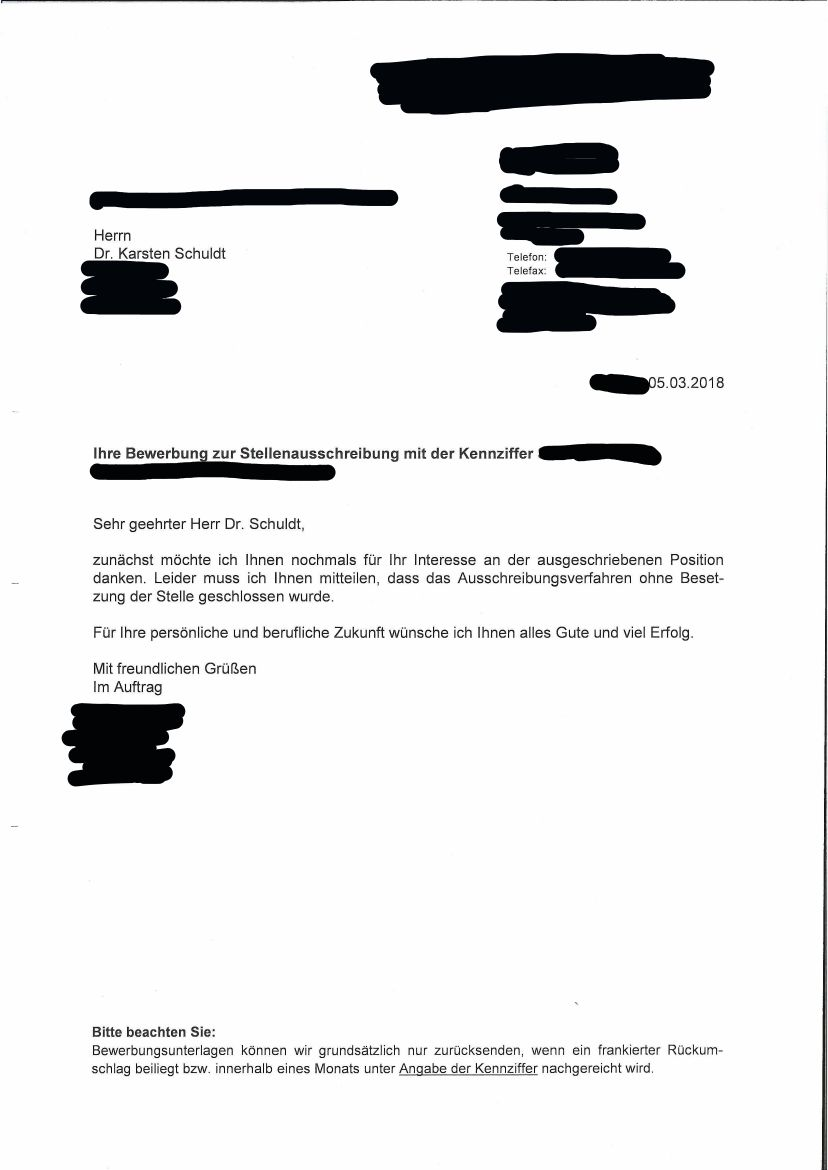
\includegraphics{img/image_1.jpg}
\caption{Ein Beispiel: Wenn eine Bibliothek eine Stelle intensiv, also
am mehreren Stellen, ausschreibt, mehrere qualifizierte Personen zum
Bewerbungsgespräch lädt, dann aber entscheidet, die Stelle lieber
unbesetzt zu lassen, haben dann vor allem die Bewerberinnen und Bewerber
versagt? Oder könnte nicht auch der Bewerbungsprozess fehlerhaft sein?
Könnten zum Beispiel die Bewerbungsgespräche gar nicht die realen
Kompetenzen der Eingeladenen aufgedeckt haben? Und was, wenn das nicht
einmal, sondern relativ oft passiert?}
\end{figure}

\begin{figure}
\centering
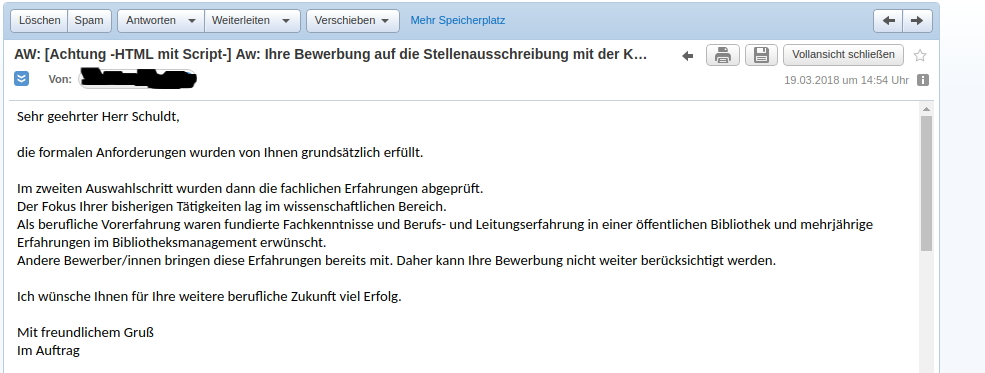
\includegraphics{img/image_2.jpg}
\caption{Ein anderes Beispiel: Wenn für eine Position in einer
Öffentlichen Bibliothek sogar jemand, der seit acht Jahren
bibliothekarisches Personal ausbildet und ständig mit und in
Bibliotheken, gerade auch Öffentlichen und Schulbibliotheken, forscht
sowie bei Strategieprozessen von Bibliotheken als Experte herangezogen
wird, als jemand eingeschätzt wird, der zu wenig Kenntnisse vom Alltag
und Management von Öffentlichen Bibliotheken hätte, was passiert dann?
Hat der Bewerber die eigenen Kompetenzen einfach falsch dargestellt? Hat
die Bibliothek ihre Erwartung zu sehr auf eine direkte Reproduktion des
eigenen Personals eingestellt, um zu sehen, was für Personal noch
möglich wäre? Schätzt sie es richtig oder falsch ein, dass dieser
Bewerber die Aufgaben in der Bibliothek nicht erfüllen können wird?
Schliesst sie damit vielleicht einfach viele ausgebildete und
interessierte Personen aus? Ist das Personalproblem -- dass sich in
diesem Fall sogar durch eine zweite Ausschreibung dieser Stelle zeigte
-- vielleicht auch ein teilweise selbst gemachtes? Und was, wenn solche
Ablehnung nicht manchmal, sondern recht oft erfolgen?}
\end{figure}

\hypertarget{eine-utopie-wie-es-wuxe4re-wenn-es-besser-wuxe4re}{%
\section*{Eine Utopie: Wie es wäre, wenn es besser
wäre}\label{eine-utopie-wie-es-wuxe4re-wenn-es-besser-wuxe4re}}

Was das Thema Arbeitsplatzkultur in Bibliotheken so schwierig zu machen
scheint, ist, dass kaum öffentlich bzw. offen darüber diskutiert wird.
Vielleicht in einigen Bibliotheken, aber nicht in allen. Und schon gar
nicht im Bibliothekswesen insgesamt. Dabei wäre ein Bibliothekswesen,
dass auch auf das Personal in den Bibliotheken achtet, dass
Möglichkeiten schafft, damit sich dieses Personal frei äussern kann und
den Eindruck hat, Dinge verändern zu können und nicht Veränderungen
einfach ausgesetzt zu sein, gewiss ein Bibliothekswesen, dass aktiver
(und attraktiver) wäre.

Wie würde ein Bibliothekswesen aussehen, dass in diesem Bezug besser
wäre? Es wäre wohl eines, welches es schätzt, wenn Personal sich
entwickeln will und dies unterstützen würde. Es wäre eines, in dem
Friktionen und Ängste offen besprochen werden können, also ein
Bibliothekswesen, in dem ehrlich über die Situation des Personals
gesprochen wird. Es wäre eines, in dem klar ist, dass in Einrichtungen
wie Bibliotheken das Personal nicht einfach (austauschbare)
Arbeitskräfte sind, sondern die individuelle Arbeit des Personals -- die
sich auch daraus bestimmt, ob es sich auf dem eigenen Arbeitsplatz gut
oder schlecht fühlt, in Kontrolle der Entwicklung oder nicht, sicher
oder nicht sicher -- die Basis für die Funktion der Bibliothek selber
darstellt. Und es wäre eines, in dem das Personal sich sinnhaft äussern
kann, also so, dass sich auch etwas ändert. Es wäre auch eines, in
welchem das Personal gewöhnt ist, sich an Entwicklungen und Diskussionen
um die zukünftige Entwicklung zu beteiligen und nicht von ihr überfahren
zu fühlen. Das heisst auch, dass es zum Arbeitsalltag gehören würde,
sich mit Fragen der Weiterentwicklung von Bibliotheken zu beschäftigen;
nicht, sich im Arbeitsalltag in den vielen Aufgaben zu verlieren und
dann keine Zeit oder kein Interesse für das Mitdenken von
Weiterentwicklungen mehr zu haben. Dabei würde Weiterentwicklung nicht
unbedingt heissen, neue Trends zu finden, sondern individuell, als
einzelne Bibliothekarin oder einzelner Bibliothekar die eigenen
Interessen an der Arbeit in der jeweiligen Bibliothek einbringen zu
können.

\hypertarget{literatur}{%
\section*{Literatur}\label{literatur}}

Alabi, Jaena (2015). Racial Microaggressions in Academic Libraries:
Results of a Survey of Minority and Non-minority Librarians. In:
\emph{The Journal of Academic Librarianship} 41 (2015) 1, 47-53,
\url{https://doi.org/10.1016/j.acalib.2014.10.008}

Carlton, Amy (2017). Fighting Sexual Harassment in the Library: Knowing
what to do when patrons go too far. In: \emph{American Libraries
Magazine The Scoop Blog}, 27.06.2017,
\url{https://americanlibrariesmagazine.org/blogs/the-scoop/fighting-sexual-harassment-library/}

Davis Kendrick, Kaetrena (2017): The Low Morale Experience of Academic
Librarians: A Phenomenological Study. In: \emph{Journal of Library
Administration} 57 (2017) 8, 846-878,
\url{https://doi.org/10.1080/01930826.2017.1368325}

Eads, Denelle (2017). Changing the Climate: Staff Development Activities
that Address the Real Issue, Communication in the Workplace. In:
\emph{North Carolina Libraries} 75 (2017) 1, 2-4,
\url{http://www.ncl.ecu.edu/index.php/NCL/article/view/739}

Eichhorn, Martin (2015). \emph{Konflikt- und Gefahrensituationen in
Bibliotheken: ein Leitfaden für die Praxis.} (3., überarbeitete Auflage)
Berlin: De Gruyter Saur, 2015

Ford, Anne (2017). Stop Sexual Harassment in Your Library: Protecting
librarians from inappropriate patrons. In: \emph{American Libraries
Magazine}, 48 (2017) 11/12, 16-17,
\url{https://americanlibrariesmagazine.org/2017/11/01/stop-sexual-harassment-your-library/}

Funge, Simon P. ; Robinson-Nkongola, Audrey ; Delancey, Laura ;
Griffiths, Austin (2017). Dropped in Without a Parachute: Library
Managers' Supervision Experiences. In: \emph{Journal of Library
Administration} 57 (2017) 7, 723-741,
\url{https://doi.org/10.1080/01930826.2017.1360021}

Hecker, Thomas E. (2007). Workplace Mobbing: A Discussion for
Librarians. In: \emph{The Journal of Academic Librarianship} 33 (2007)
4, 439-445, \url{https://doi.org/10.1016/j.acalib.2007.03.003}

Houston, Cynthia ; Paganelli, Andrea (2015). An Exploratory Study of
School Librarians' Emotional Response to Change in the Workplace. In:
\emph{Libres} 25 (2015) 1, 16-32,
\url{https://www.libres-ejournal.info/1586}

Henry, Jo ; Eshleman, Joe ; Moniz, Richard (2018). \emph{The
Dysfunctional Library: Challenges and solutions to workplace
relationships}. Chicago: ALA Editions, 2018

Henry, Jo ; Eshlemann, Joe ; Croxton, Rebecca ; Moniz, Richard (2018).
Incivility and Dysfunction in the Library Workplace: Perceptions and
Feedback from the Field. In: \emph{Journal of Library Administration} 58
(2018) 2, 128-152, \url{https://doi.org/10.1080/01930826.2017.1412708}

Kaba, Abdoulaye (2017). Library employment: Satisfaction, opportunities,
challenges, and future actions as perceived by academic librarians. In:
\emph{Library Management} 38 (2017) 8/9, 511-527,
\url{https://doi.org/10.1108/LM-03-2017-0036}

Leiding, Reba (2010). Mobbing in the library workplace: What it is and
how to prevent it. In: \emph{College \& Research Libraries News} 71
(2010) 7, \url{https://doi.org/10.5860/crln.71.7.8406}

Morgan, Chad (2014). Craft and Librarianship: A Reconsidertation of the
Sources of Librarian Job Satisfaction. In: \emph{Journal of Library
Administration} 54 (2014) 8, 637-658, ,
\url{https://doi.org/10.1080/01930826.2014.965096}

Neville, Tina M. ; Henry, Deborah B. (2017). Career Plateauing among
Senior Librarians. In: \emph{Journal of Library Administration} 57
(2017) 6, 651-673, \url{https://doi.org/10.1080/01930826.2017.1337971}

Oyovwe Tinuoye, Gloria O. ; Omeluzor, Saturday U. ; Oji Akpojotor, Lucky
(2016). Factors influencing job satisfaction of academic librarians in
university libraries in Edo and Delta states, Nigeria. In: \emph{The
Electronic Library} 34 (2016) 6, 985-996,
\url{https://doi.org/10.1108/EL-07-2015-0128}

Peet, Lisa (2017). Joy Doan and Ahmed Alwan: Examining Status
Microaggressions and Academic Libraries. In: \emph{Library Journal}
27.April 2017,
\url{http://lj.libraryjournal.com/2017/04/academic-libraries/joy-doan-and-ahmed-alwan-examining-status-microaggressions-and-academic-libraries}

Ryan, Marianne (2016). Besting the Workplace Bully. In: \emph{Reference
\& User Services Quarterly} 55 (2016) 4, 267-269,
\url{https://doi.org/10.5860/rusq.55n4.267}

Wheeler, Ronald (2016). About Microaggressions. In: \emph{Law Library
Journal} 108 (2016) 2, 321-329

%autor
\begin{center}\rule{0.5\linewidth}{\linethickness}\end{center}

\textbf{Karsten Schuldt}, Berlin / Chur, ist Redakteur der LIBREAS.
Library Ideas und Wissenschaftlicher Mitarbeiter am Schweizerischen
Institut für Informationswissenschaft, HTW Chur.

\end{document}
